\chapter{Path and Navigation}
\section{Path system}\label{Ch:LandingPath}
The path system is designed to enable \gls{uav} landing in both a stationary and a moving net. The path is created in two main stages. The first is the creation of the landing path, which is defined as a straight line along the heading of the net, as shown in figure \ref{Fig:LandingPhase}. The second stage is the approach path, which apply a lateral Dubins path and longitudinal straight line path to create a path that ensures that the \gls{uav} is able to enter the landing path at the correct height and attitude.
\subsection{Landing Path}\label{SS:netApproach}
The landing path is inspired by the work done in \citep{Skulstad&Syversen} where waypoint was used to create a straight line path towards the net. This method proved successful, and since the \gls{uav} descent towards the net should be as controlled as possible only small angles is used when transitioning between way-points. The straight line path is constructed relative to the net as shown in figure \ref{Fig:LandingPhase}, with way-points given as:
\begin{subequations}
\begin{align}
&\mathbf{WP4} = 
\begin{bmatrix}
-a0 \\
0 \\
h_{nc} + a1\tan(\gamma_a) 
\end{bmatrix}\\
&\mathbf{WP3} = 
\begin{bmatrix}
a1 \\
0 \\
h_{nc} - a1\tan(\gamma_a)
\end{bmatrix}\\
&\mathbf{WP2} = \mathbf{WP3} + 
\begin{bmatrix}
a2 \\
0 \\
a2\tan(\gamma_d)
\end{bmatrix}\\
&\mathbf{WP1} = \mathbf{WP2} + 
\begin{bmatrix}
a3 \\
0 \\
0 \\
\end{bmatrix}
\end{align}
\end{subequations}
were the description of the parameters used is given in table \ref{Tb:Approach Parameters}. The net is placed between the fourth and third way points such that transitional behaviour do not occur during the finale stage of the net landing. In addition the path has been made with the assumption that the $\gamma_a$ and $\gamma_d$ is considered small. This assumption is made to ease the demand of the controllers used in the landing system.
\begin{table}[H]
\begin{center}
    \begin{tabular}{ | l | l |}
    \hline
    \textbf{Parameter} & \textbf{Description} \\ \hline
    $h_{nc}$ & The height from ground to the net center \\ \hline
    $a0$ & The distance behind the net \\ \hline
    $a1$ & The distance in front of the net \\ \hline
    $a2$ & The length of the glide slope \\ \hline
    $a3$ & The length of the approach towards the glide slope \\ \hline
    $\gamma_a$ & The net attack angle \\ \hline
    $\gamma_d$ & The glide slope angle \\ \hline
    \end{tabular}
\end{center}
\caption{Net approach parameters }
\label{Tb:Approach Parameters}
\end{table}
The way point vectors are rotated into the NED frame by a rotation around the z-axes.
\begin{equation}
\mathbf{WP}^n = \mathbf{R}(\psi_{net})\mathbf{WP}^b
\end{equation}
were $\psi_{net}$ is the heading of the net, and $\mathbf{R}(\psi_{net})$ is the rotation matrix around the z-axis.
\begin{figure}
\def\svgwidth{\textwidth} % Defining the width since Inkscape hasn't done this yet in the .pdf_tex file
\input{InkFig/LandingPhase.pdf_tex}
\caption{The virtual runway}
\label{Fig:LandingPhase}
\end{figure}

\subsection{Approach path}\label{SS:LandingApproach}
The landing path is separated into two parts, which is a lateral and longitudinal path. The path is designed to ensure that the \gls{uav} follows the path along the virtual runway it must be at the correct height with the correct attitude from any initial position. In addition it's desirable that the decent angle is kept small to ease the strain on the control system, and reduce chance of overshoot of way-points.
\subsubsection{Lateral path}
The lateral path is designed as a Dubins path, where the initial position is the start pose, $P_s$, and the final pose $P_f$ is the start of the landing path. Dubins path was chosen due to it's simplicity in description and it fulfils the requirement that it's smooth enough for path following.

The lateral path is constructed following the equations in section \ref{S:DubinsPath}, however the rotation direction in each circle must first be determined. The desired behaviour is to find the shortest path of the four different variants given in table \ref{Tb:DubinsTurningDirection}. The shortest path is determined by calculating the length of each variants, where the shortest is chosen. The resulting the path is shown in figure \ref{Fig:LateralPath}.
\begin{figure}[H]
	\centering
		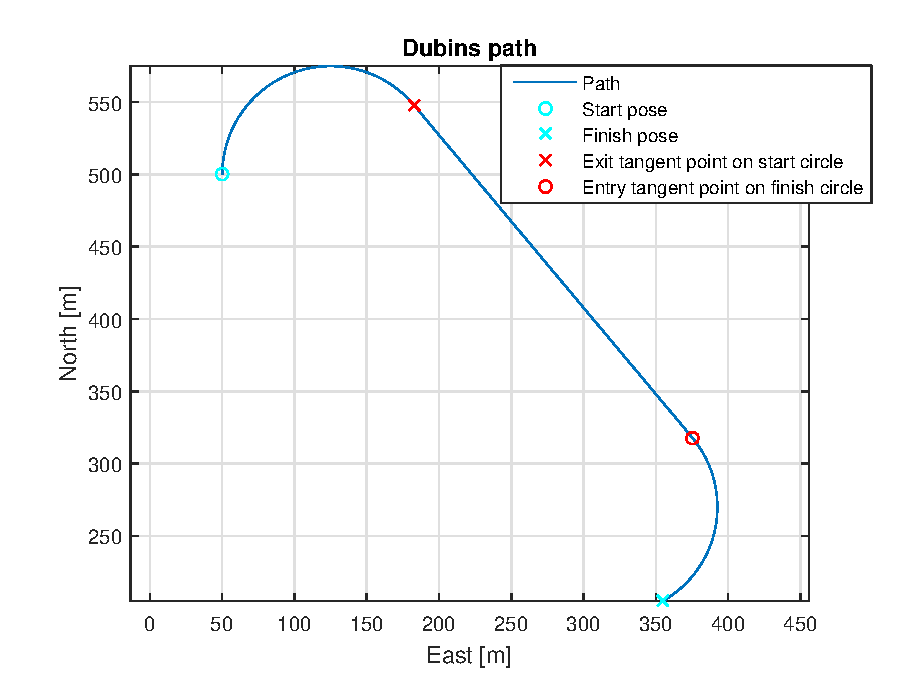
\includegraphics[width=1\textwidth]{figs/SysPlot/DubinsPath.eps}
		\caption{Lateral Dubins path}
		\label{Fig:LateralPath}
\end{figure}

\begin{subequations}
\begin{align}
\psi_0 &= \begin{cases}
\atan2(Y_s-Y_{cs},X_s-X_{cs}) & \text{if start circle} \\
\atan2(Y_{P_N}-Y_{cf},X_{P_N}-X_{cf}) & \text{otherwise}
\end{cases}\\
\psi_1 &= \begin{cases}
\atan2(Y_{P_\chi}-Y_{cs},X_{P_{\chi}}-X_{cs}) & \text{if start circle} \\
\atan2(Y_{f}-Y_{cf},X_{f}-X_{cf}) & \text{otherwise}
\end{cases}
\end{align}
\end{subequations}

\begin{equation}
\psi_{max} = \begin{cases}
-|\psi_1 - \psi_0| & \text{if counter clockwise rotation and } \psi_1 - \psi_0 \leq 0 \\
-(2\pi - |\psi_1-\psi_0|) & \text{ if counter clockwise rotation and } \psi_1 - \psi_0 > 0 \\
|\psi_1 - \psi_0| & \text{if clockwise rotation and } \psi_1 - \psi_0 \geq 0 \\
(2\pi - |\psi_1-\psi_0|) & \text{ if clockwise rotation and } \psi_1 - \psi_0 < 0
\end{cases}
\end{equation}
where $psi_1-\psi_0 \in(-\pi,\pi]$.
\begin{subequations}
\begin{align}
h &= \frac{d_{arc}}{R} \\
N &= \ceil[\Bigg]{\frac{\text{sign}(\psi_{max})\psi_{max}}{h}} + 1 \\
h &= \text{sign}(\psi_{max})h
\end{align}
\end{subequations}
where $h$ is arc angle step and $N$ the total number of steps in the arc.
\begin{equation}
\psi(\varpi) = \begin{cases}
\psi_{max} & \varpi = N-1 \\
\varpi h & \text{otherwise}
\end{cases}
\end{equation}
where $\varpi = 1,...,N-1$.
\begin{equation}
\mathbf{r}(\varpi) = \begin{bmatrix}
\mathbf{O}_c \\
0
\end{bmatrix} + R\begin{bmatrix}
\cos(\psi_0 + \psi(\varpi)) \\
\sin(\psi_0 + \psi(\varpi)) \\
0
\end{bmatrix}
\end{equation}

\subsubsection{Longitudinal path}
The longitudinal path is designed as a straight line along the lateral path, which results in a spiral path in the arcs created by the lateral path. The path hold a constant decent angle until the correct height is reached, which is defined as the start height for the virtual runway. The resulting height profile of the approach path becomes a straight line path shown in figure \ref{Fig:HeightProfile}. The longitudinal path is given as:
\begin{equation}
r(i+1) = r(i) +
\begin{bmatrix}
0\\
0\\
||p(i)||_2\tan(\gamma_d)
\end{bmatrix}
\end{equation}
where $r(i)$ is the landing path and 
$p = \begin{bmatrix}
x(i) & y(i)
\end{bmatrix}^T$ is the lateral path. During each iteration the algorithm checks if the next step can reach the correct height with a decent angel greater or equal to the maximum decent angel $\gamma_d$. In the case where the the height at the end of the lateral path is not the same height as the start height for the virtual runway, the landing path will enter a spiral which decent towards the correct height. The spiral is centred in the same circle that is used to create the arc for the final turn in the lateral path. The spiral is exited when the correct height is reached, and a arc is created from the spiral exit point towards the lateral path final point.

The height profile of the landing path is shown in figure \ref{Fig:HeightProfile},with the resulting path connected to the virtual runway shown in figure \ref{Ch:LandingPath}.

\begin{figure}[H]
	\centering
		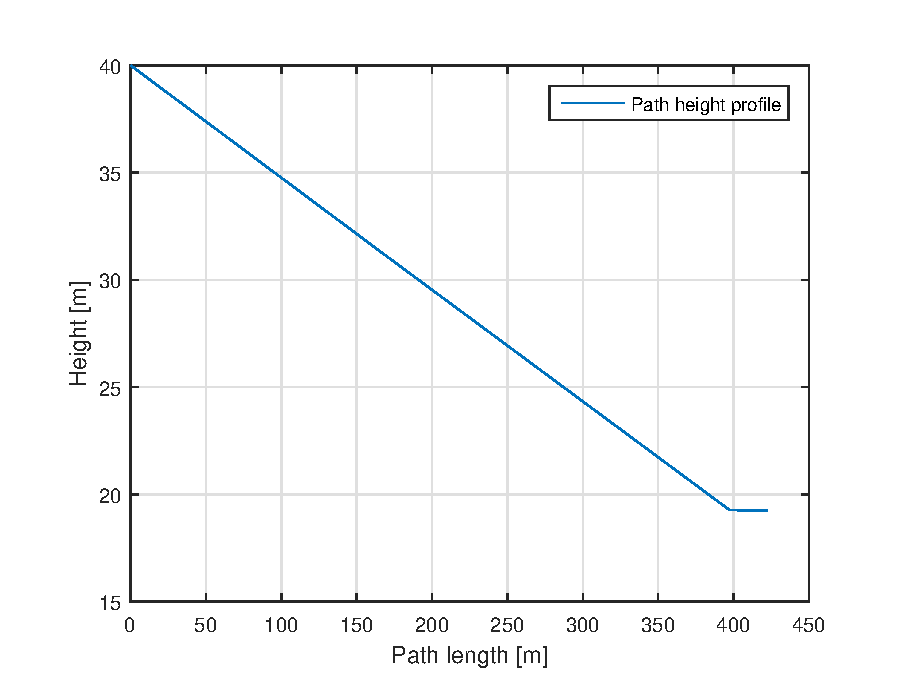
\includegraphics[width=1\textwidth]{figs/SysPlot/heightProfile.eps}
		\caption{Height profile of the landing path}
		\label{Fig:HeightProfile}
\end{figure}

\begin{figure}[H]
	\centering
		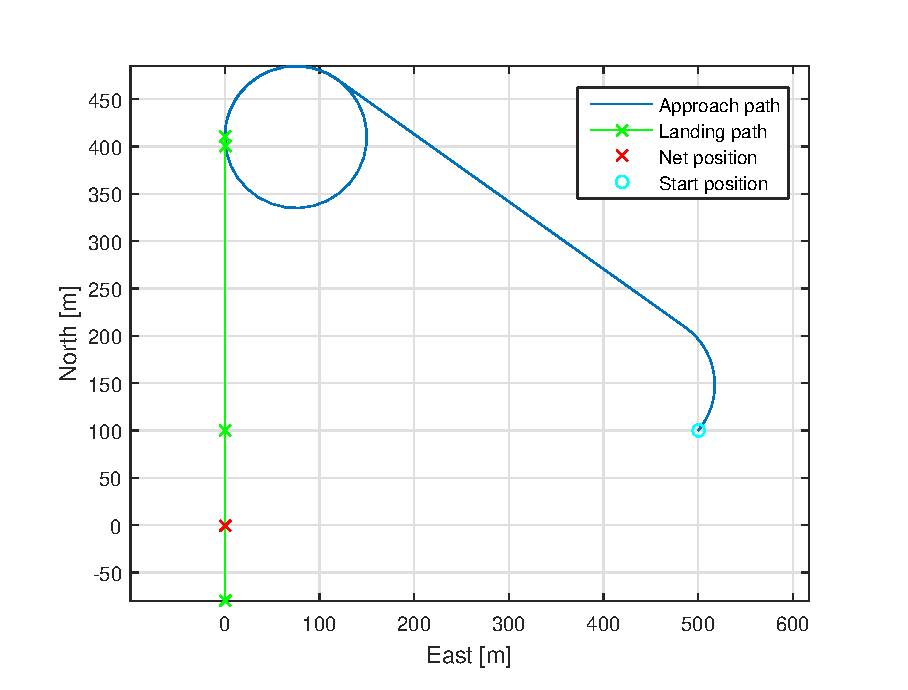
\includegraphics[width=1\textwidth]{figs/SysPlot/LandingPath.eps}
		\caption{Landing path connected to the virtual runway}
		\label{Fig:LandingPath}
\end{figure}

\section{Navigation system}
The navigation system apply \gls{rtk-gps} for position and velocity measurement, which provide higher position accuracy then a standalone \gls{gps}. However the \gls{rtk-gps} is subject to drop out, which create a situation where the navigation system should switch to standalone \gls{gps} or wait for the \gls{rtk-gps} to return. A state machine has been created to handle the state switching between \gls{rtk-gps} and the external navigation data, which is navigation data from the Pixhawk. This is handled in two steps. The first is a short loss compensator stage, where the backup standalone \gls{gps} is compensated to get a position solution closer to the \gls{rtk-gps} solution. The second stage fully disconnect the \gls{rtk-gps}.
\subsection{Navigation state}\label{S:NavState}
The navigation system consists of five states, which is controlled by a state machine. The state transitions are determined by what's available and what the operator has specified should be used. The output from the state machine is the IMC message EstimatedState, which is the only state source used in the Dune system. The state machine also dispatch a IMC message that informs which the source used in the navigation system, and which sources is available. Currently only the \gls{rtk-gps} system is considered as a internal system, however this can be expanded to include other sensors used in the Dune system.

The input to the navigation system is IMC message ExternalNav and GpsRtkFix. The ExternalNav message is the primary state source when the \gls{rtk-gps} is not in use, and it's receive the state information from the Pixhawk mounted in the X8.

During a short loss of the \gls{rtk-gps} the position solution in the ExternalNav message is compensated to avoid sudden change in position. The short loss compensator is explain further in \ref{ss:ShortLoss}. The short loss system is implemented to avoid drop out of the \gls{rtk-gps} when a message is delayed, or its struggling due to the dynamic behaviour of the \gls{uav}.

The state machine is depicted in figure \ref{Fig:NavState}, with the edge description given in table \ref{Tb:Nav state edge}.

\begin{figure}\label{Fig:NavState}
\def\svgwidth{\textwidth} % Defining the width since Inkscape hasn't done this yet in the .pdf_tex file
\input{InkFig/StateMachine.pdf_tex}
\end{figure}
\begin{table}[H]

    \begin{tabular}{ | p{1cm} | p{8cm} | | p{4cm} |}
    \hline
    \textbf{Edge} 	& \textbf{Event} 										& \textbf{Guard} \\ \hline
    A 				& Event: Received External Nav message 					& None \\ \hline
    B 				& Time out: Fix \gls{rtk-gps} solution for $x$ seconds 	& None \\ \hline
    C 				& Time out: $x$ seconds since last valid GpsFixRtk 		& None \\ \hline
    D 				& Flag: Using Rtk is set true& None \\ \hline
    E 				& Flag: Using Rtk is set false& None \\ \hline
    F 				& Time out: $x$ seconds since last valid GpsFixRtk 		& Short loss compensator:\\ 
      				& Event: Received GpsRtkFix with $type==None$ 			& Enabled\\ \hline
    G 				& Event: Received valid GpsFixRtk message				& None \\ \hline
    H 				& Time out: $x$ seconds since last valid GpsFixRtk 		& Short loss compensator:\\
    				& Event: Received GpsRtkFix with $type==None$			& Disabled \\ \hline
    I 				& Time out: $x$ seconds since last valid GpsFixRtk 		& None \\ \hline
    \end{tabular}

\caption{Net approach parameters }
\label{Tb:Nav state edge}
\end{table}

\begin{table}
\begin{tabular}{ | p{3cm} | p{8cm} |}
	\hline 
	\textbf{State}						& \textbf{Description} \\ \hline
	Initialize							& The task starting up\\ \hline
	Using external						& The navigation task apply the external navigation source in the state message\\ \hline
	RTK ready							& The \gls{rtk-gps} is ready for use, however the external navigation source is still used\\ \hline
	Using RTK							& The navigation task apply the \gls{rtk-gps} in the state message\\ \hline
	Using short RTK loss compensator	& The navigation task apply the external navigation source with a compensation term to reduce the effect of \gls{rtk-gps} loss. \\ \hline
\end{tabular}
\end{table}
\subsubsection{Short loss of RTKGPS}\label{ss:ShortLoss}
In the event of \gls{rtk-gps} drop out a offset can be added to the position solution in order to prevent a sudden change in position. The offset is defined as the average difference between the $N$ latest position solution from the \gls{rtk-gps} and the external navigation system:
\begin{equation}
offset = \frac{1}{N}\sum_{n=0}^N(RTKGPS(n)-External(n))
\end{equation}
where the \gls{rtk-gps} solution is displaced into the External nav system. However during the implantation it was discovered that the standard displace function in the DUNE literary was inaccurate in correctly calculating the hight of a offset point. The problem was that the geodetic latitude calculation was calculate assuming that the Earth has a spheric shape. This was solved by creating a new displace function where the geodetic latitude is calculated in according to